\section{Implementation}

While implementing the project, I broke down the large task of making a reinforcement learning agent to play pokemon red into smaller tasks. The first step was to create or find an environment that was an accurate depiction or an environment wrapping around the pokemon game itself. After finding the environment, I would have check the details of the environment and make sure it was compatible with the different algorithms I would be using. Once an environment and reinforcement learning algorithm was chosen, I was able to achieve a minimum viable product by training a single agent to play the game and defeat the first gym. After this, I would be able to scale up the project by finding methods to accelerate the training of the agent without sacrificing the quality of the agent's performance and amount of timesteps it was training for. 

\subsection{Environment}



\subsection{Reward Function}

\subsection{Navigation}

\subsection{Combat}

\subsection{Agent training}

In order to scale up the project to accelerate the training of the agent, the speed at which the emulation was running was increased. This was done using Pyboy's emulation speed-up function and editing the rate at which screen information and RAM was read to stay in sync with the emulation. This allowed the agent to train at a faster rate, without making any sacrifices to the quality of the agent's training. The emulation was sped up by a rate of 6x because this was the fastest rate at which the environment was able to stay in sync with the emulation. Due to the environment not being a recreation of the original game and instead extract information and applying input to the environment, the environment and emulation had to stay in sync so that information was being extracted and injected at the correct moments.

Another technique used to accelerate the training of the agent was to train the agent in parallel. This was done using the 'SubprocVecEnv' function from the 'stablebaselines3' library. A total of 11 instances of the environment were trained in parallel because this was the maximum amount of instances that the hardware I had easy access to could handle. The hardware used to train the agent is specified in \ref{subsec:Hardware} Hardware Requirements. 11 instances of parallel traning was chosen because it was the maximum amount allowed to be trained on with 64 GB of RAM before the system would crash due to memory issues when updating the policy at the end of every episode. 

In addition, using gymnasium's 'headless' function allowed the agent to train without the need to render the game, which lowered the system requirements to train. Lowering the hardware requirements to train the agent allows the potential of more instances of the environment to be trained in parallel, which would allow the agent to train at a faster rate.

While training the agent, the hardware component that was bottlenecking further instances of the environment being trained in parallel was the RAM. Training did not have that high of a GPU nor CPU requirement. This is evident in the graphs below. 

\begin{figure}[H]
    \centering
    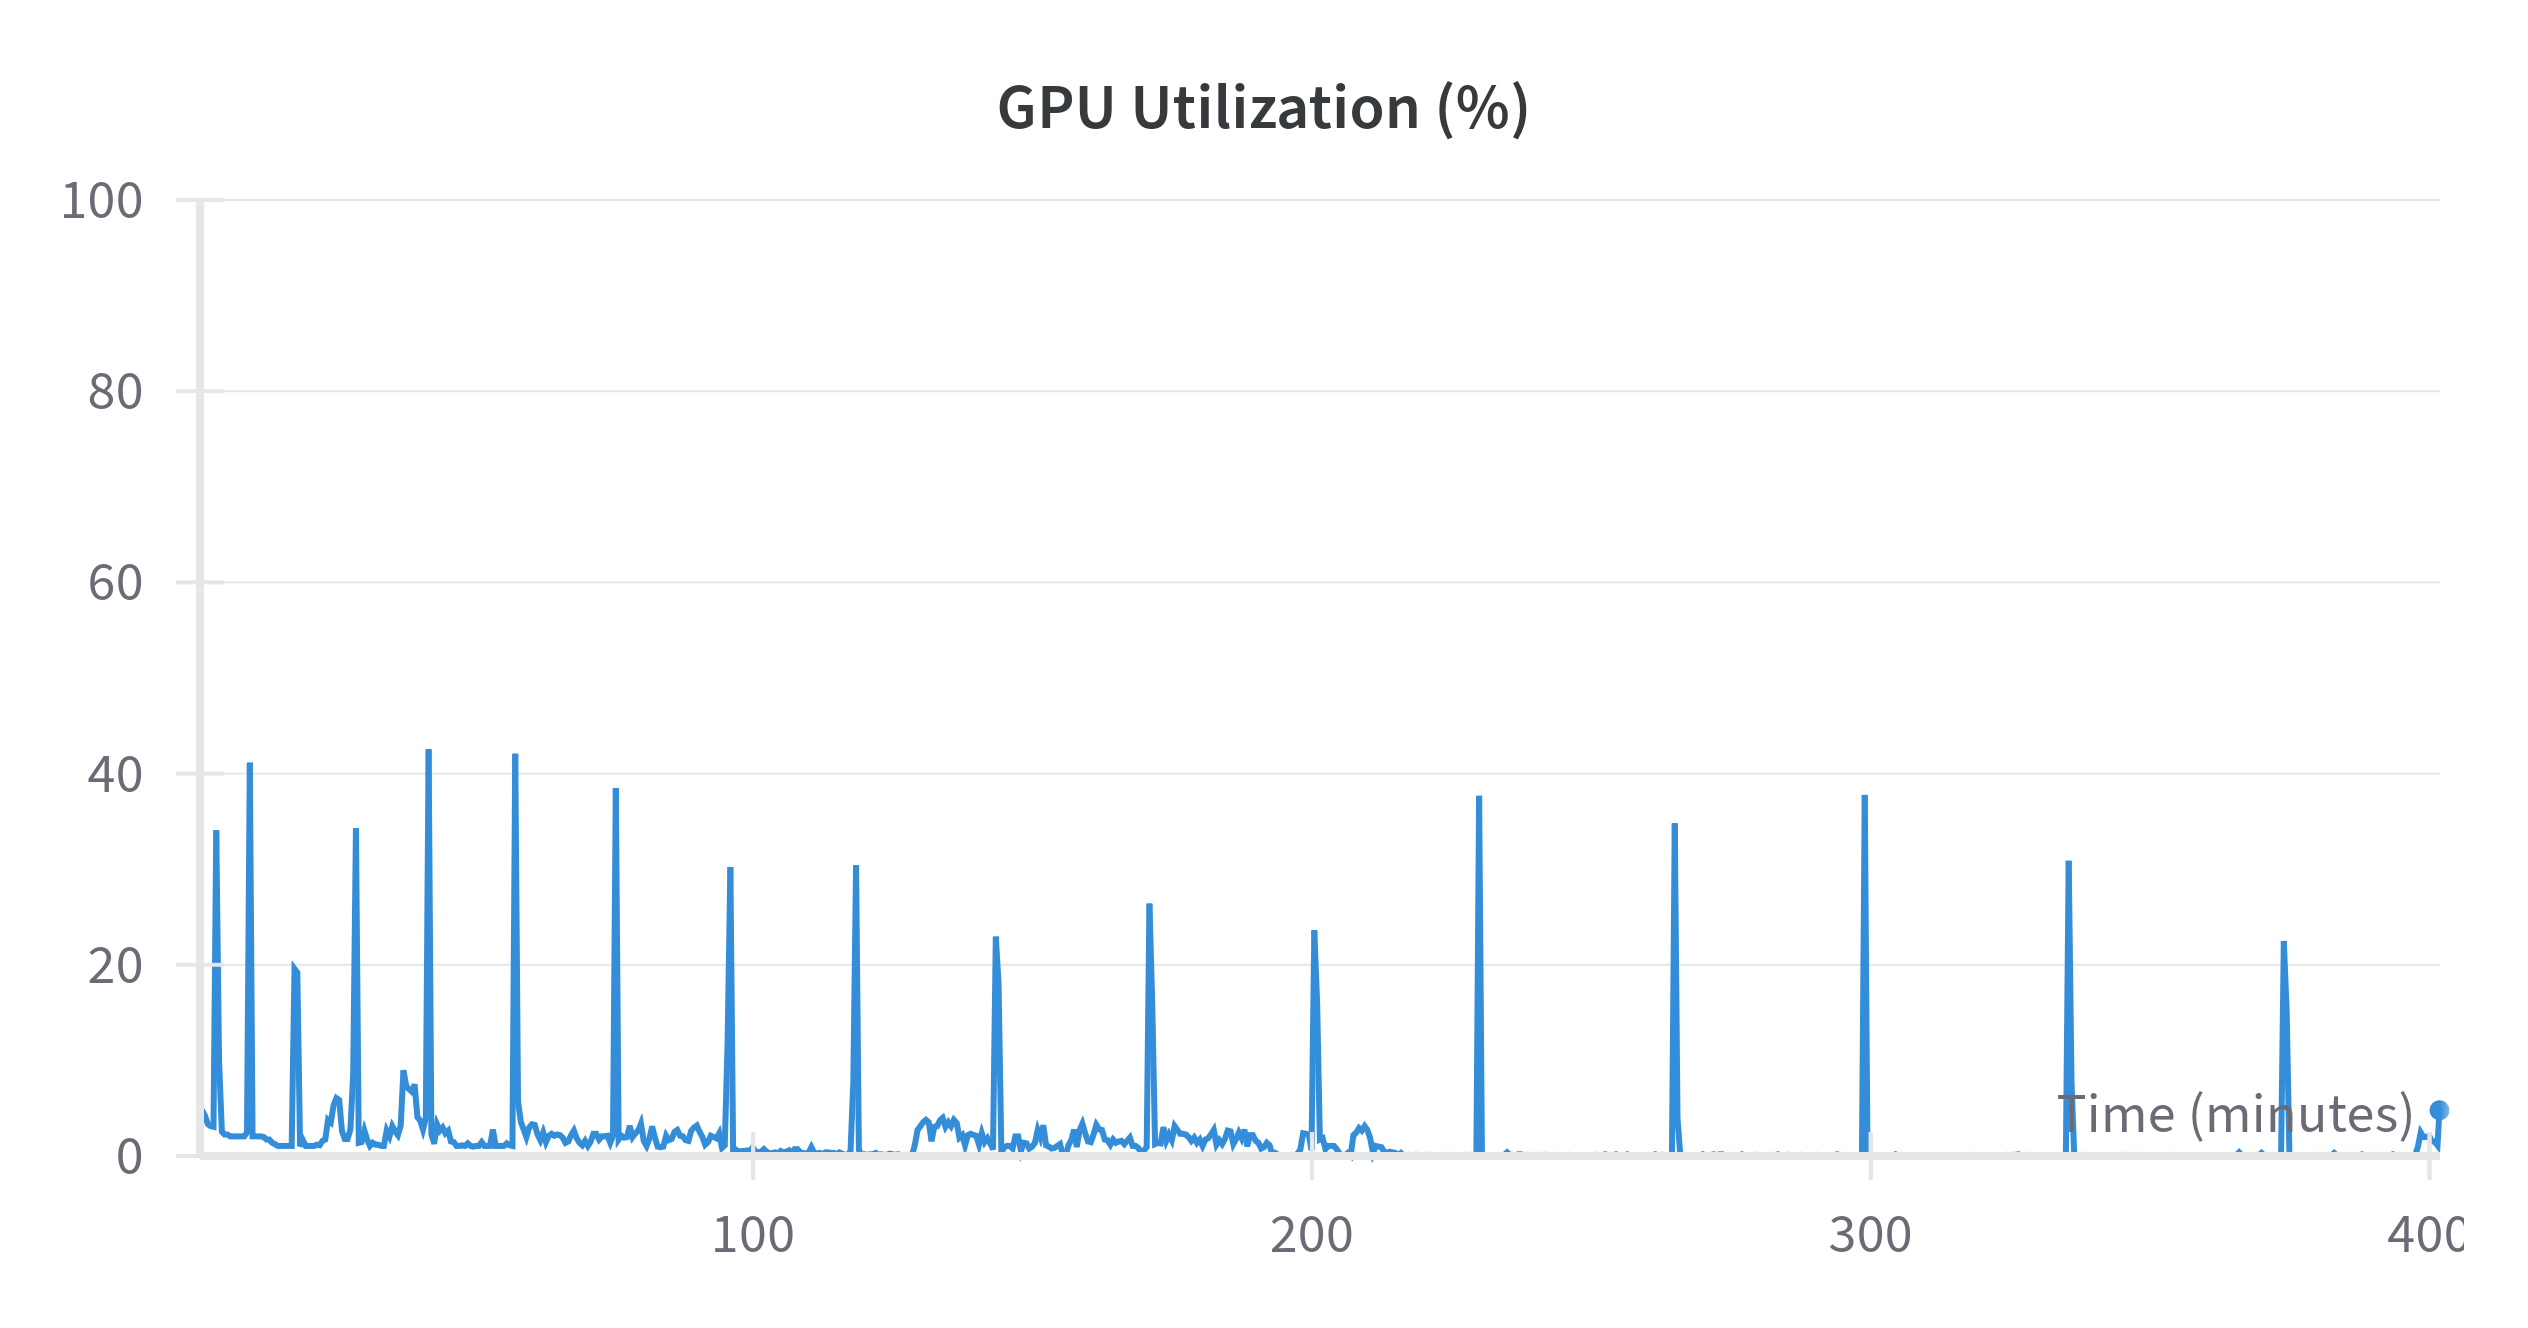
\includegraphics[width=0.8\textwidth]{figures/GPU_Utilization.png}
    \caption{GPU percentage usage while training an agent}
    \label{fig:gpu_memory_usage}
\end{figure}

\begin{figure}[H]
    \centering
    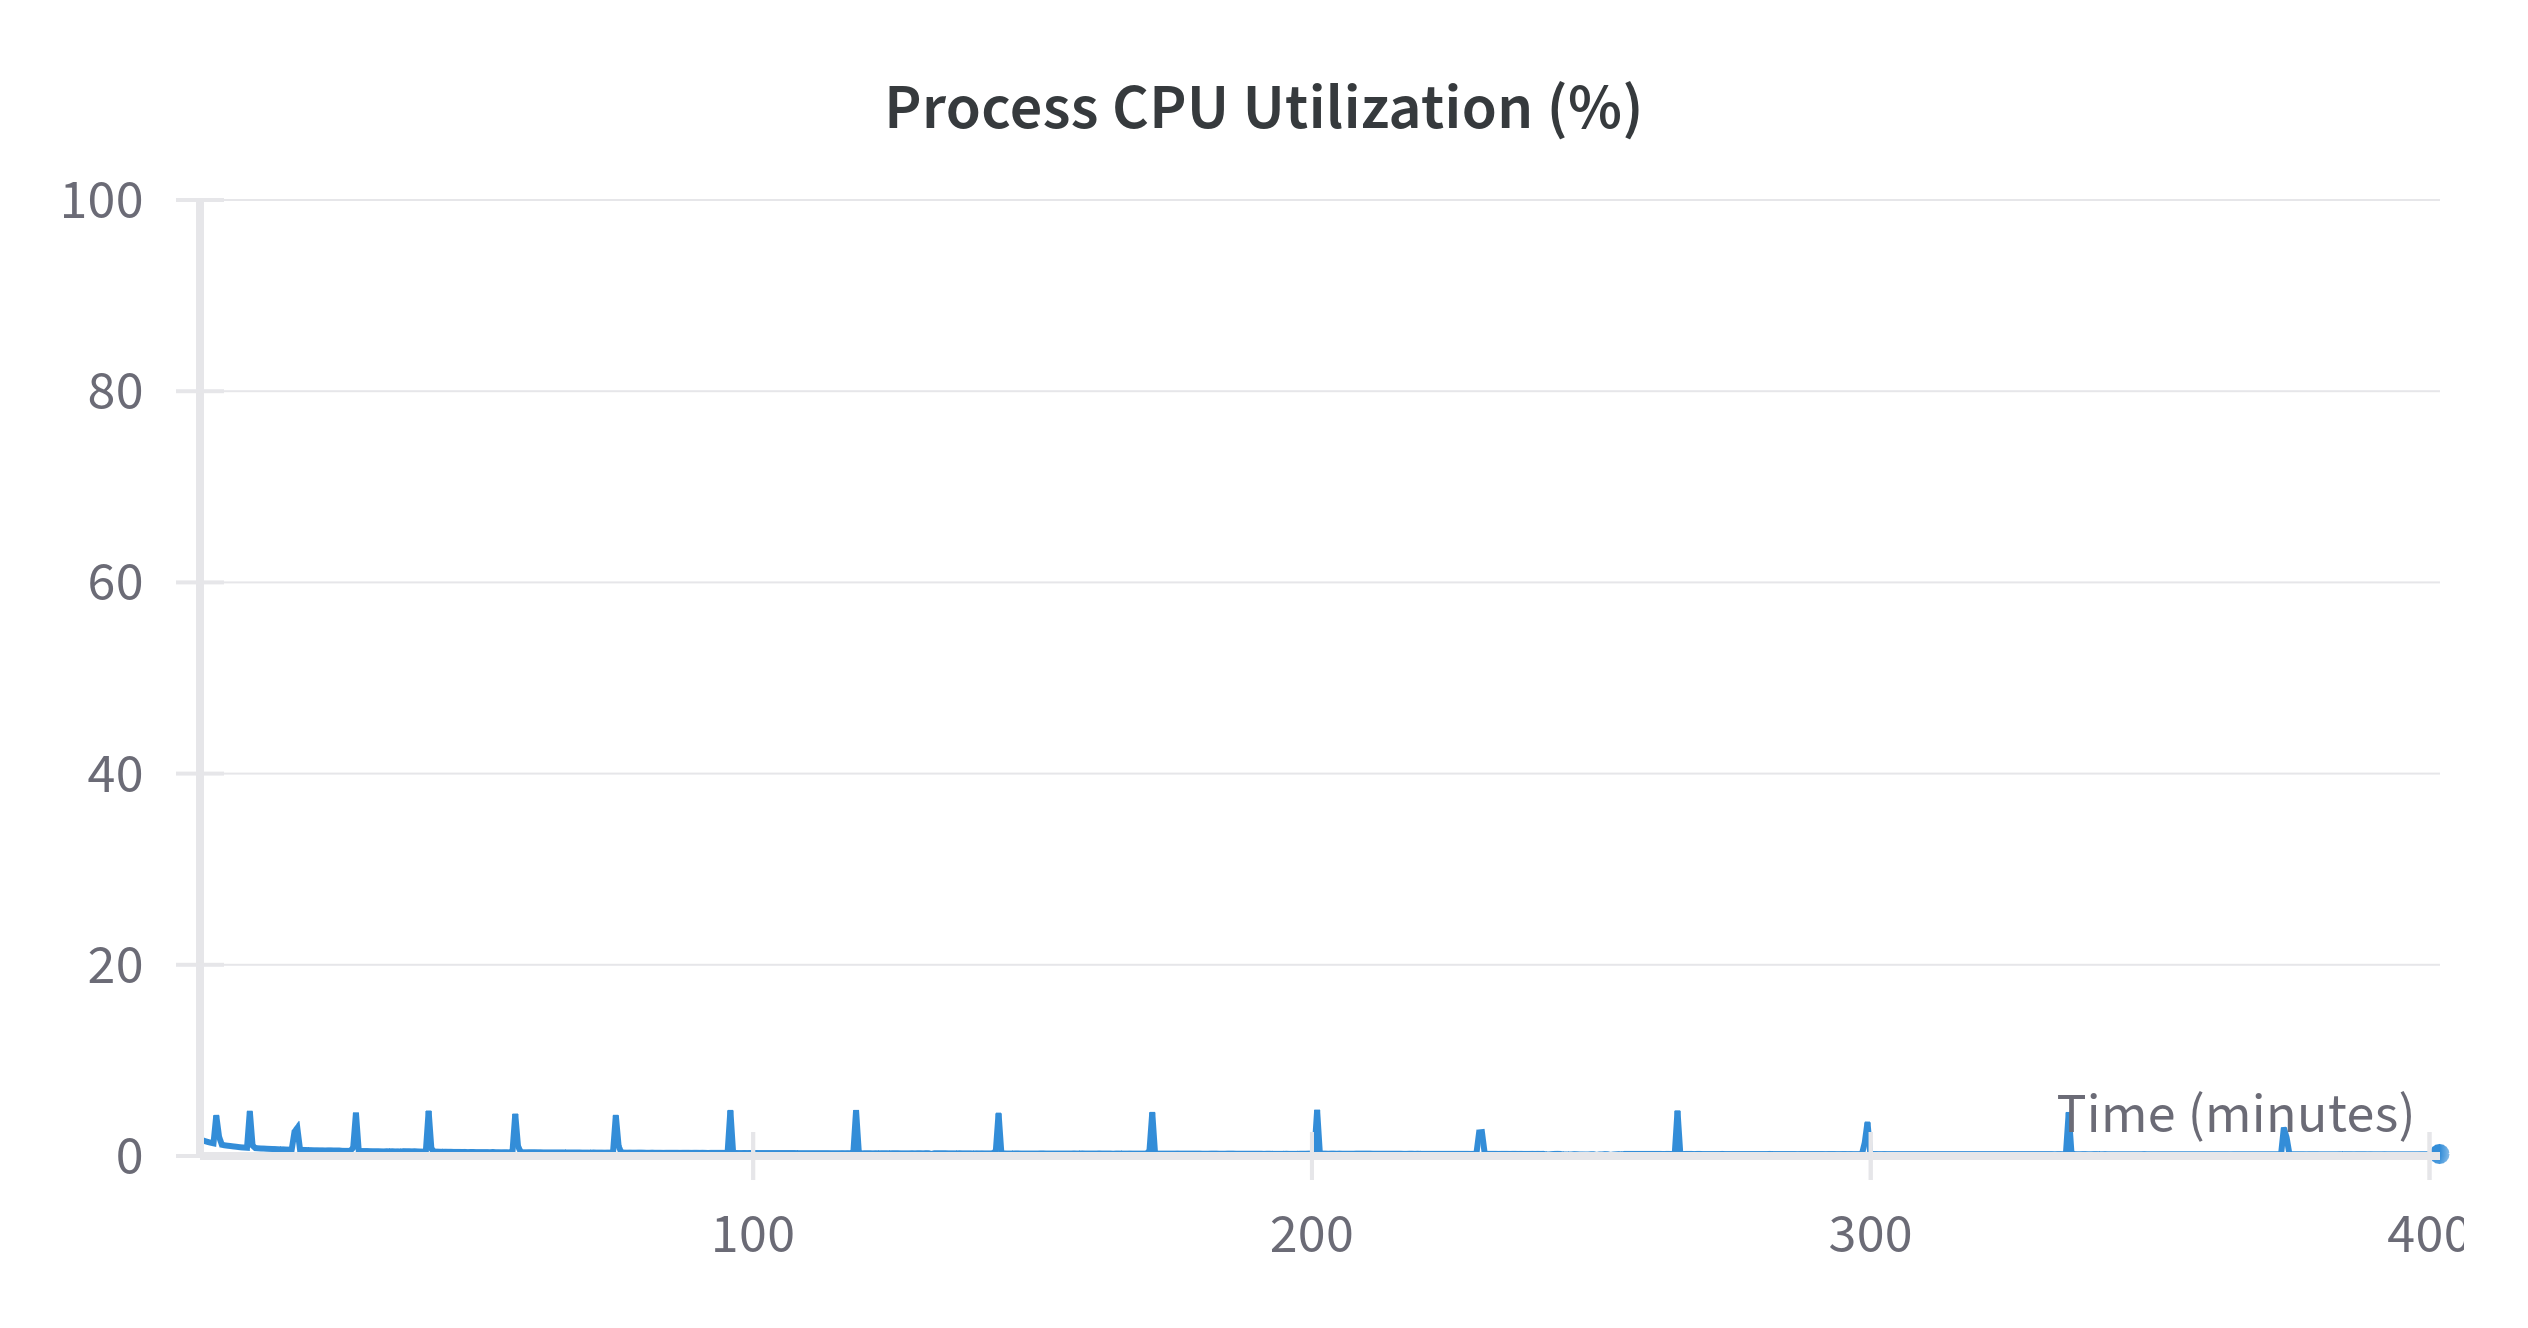
\includegraphics[width=0.8\textwidth]{figures/total_cpu_utilization.png}
    \caption{Total CPU usage while training an agent}
    \label{fig:ram_usage}
\end{figure}

\begin{figure}[H]
    \centering
    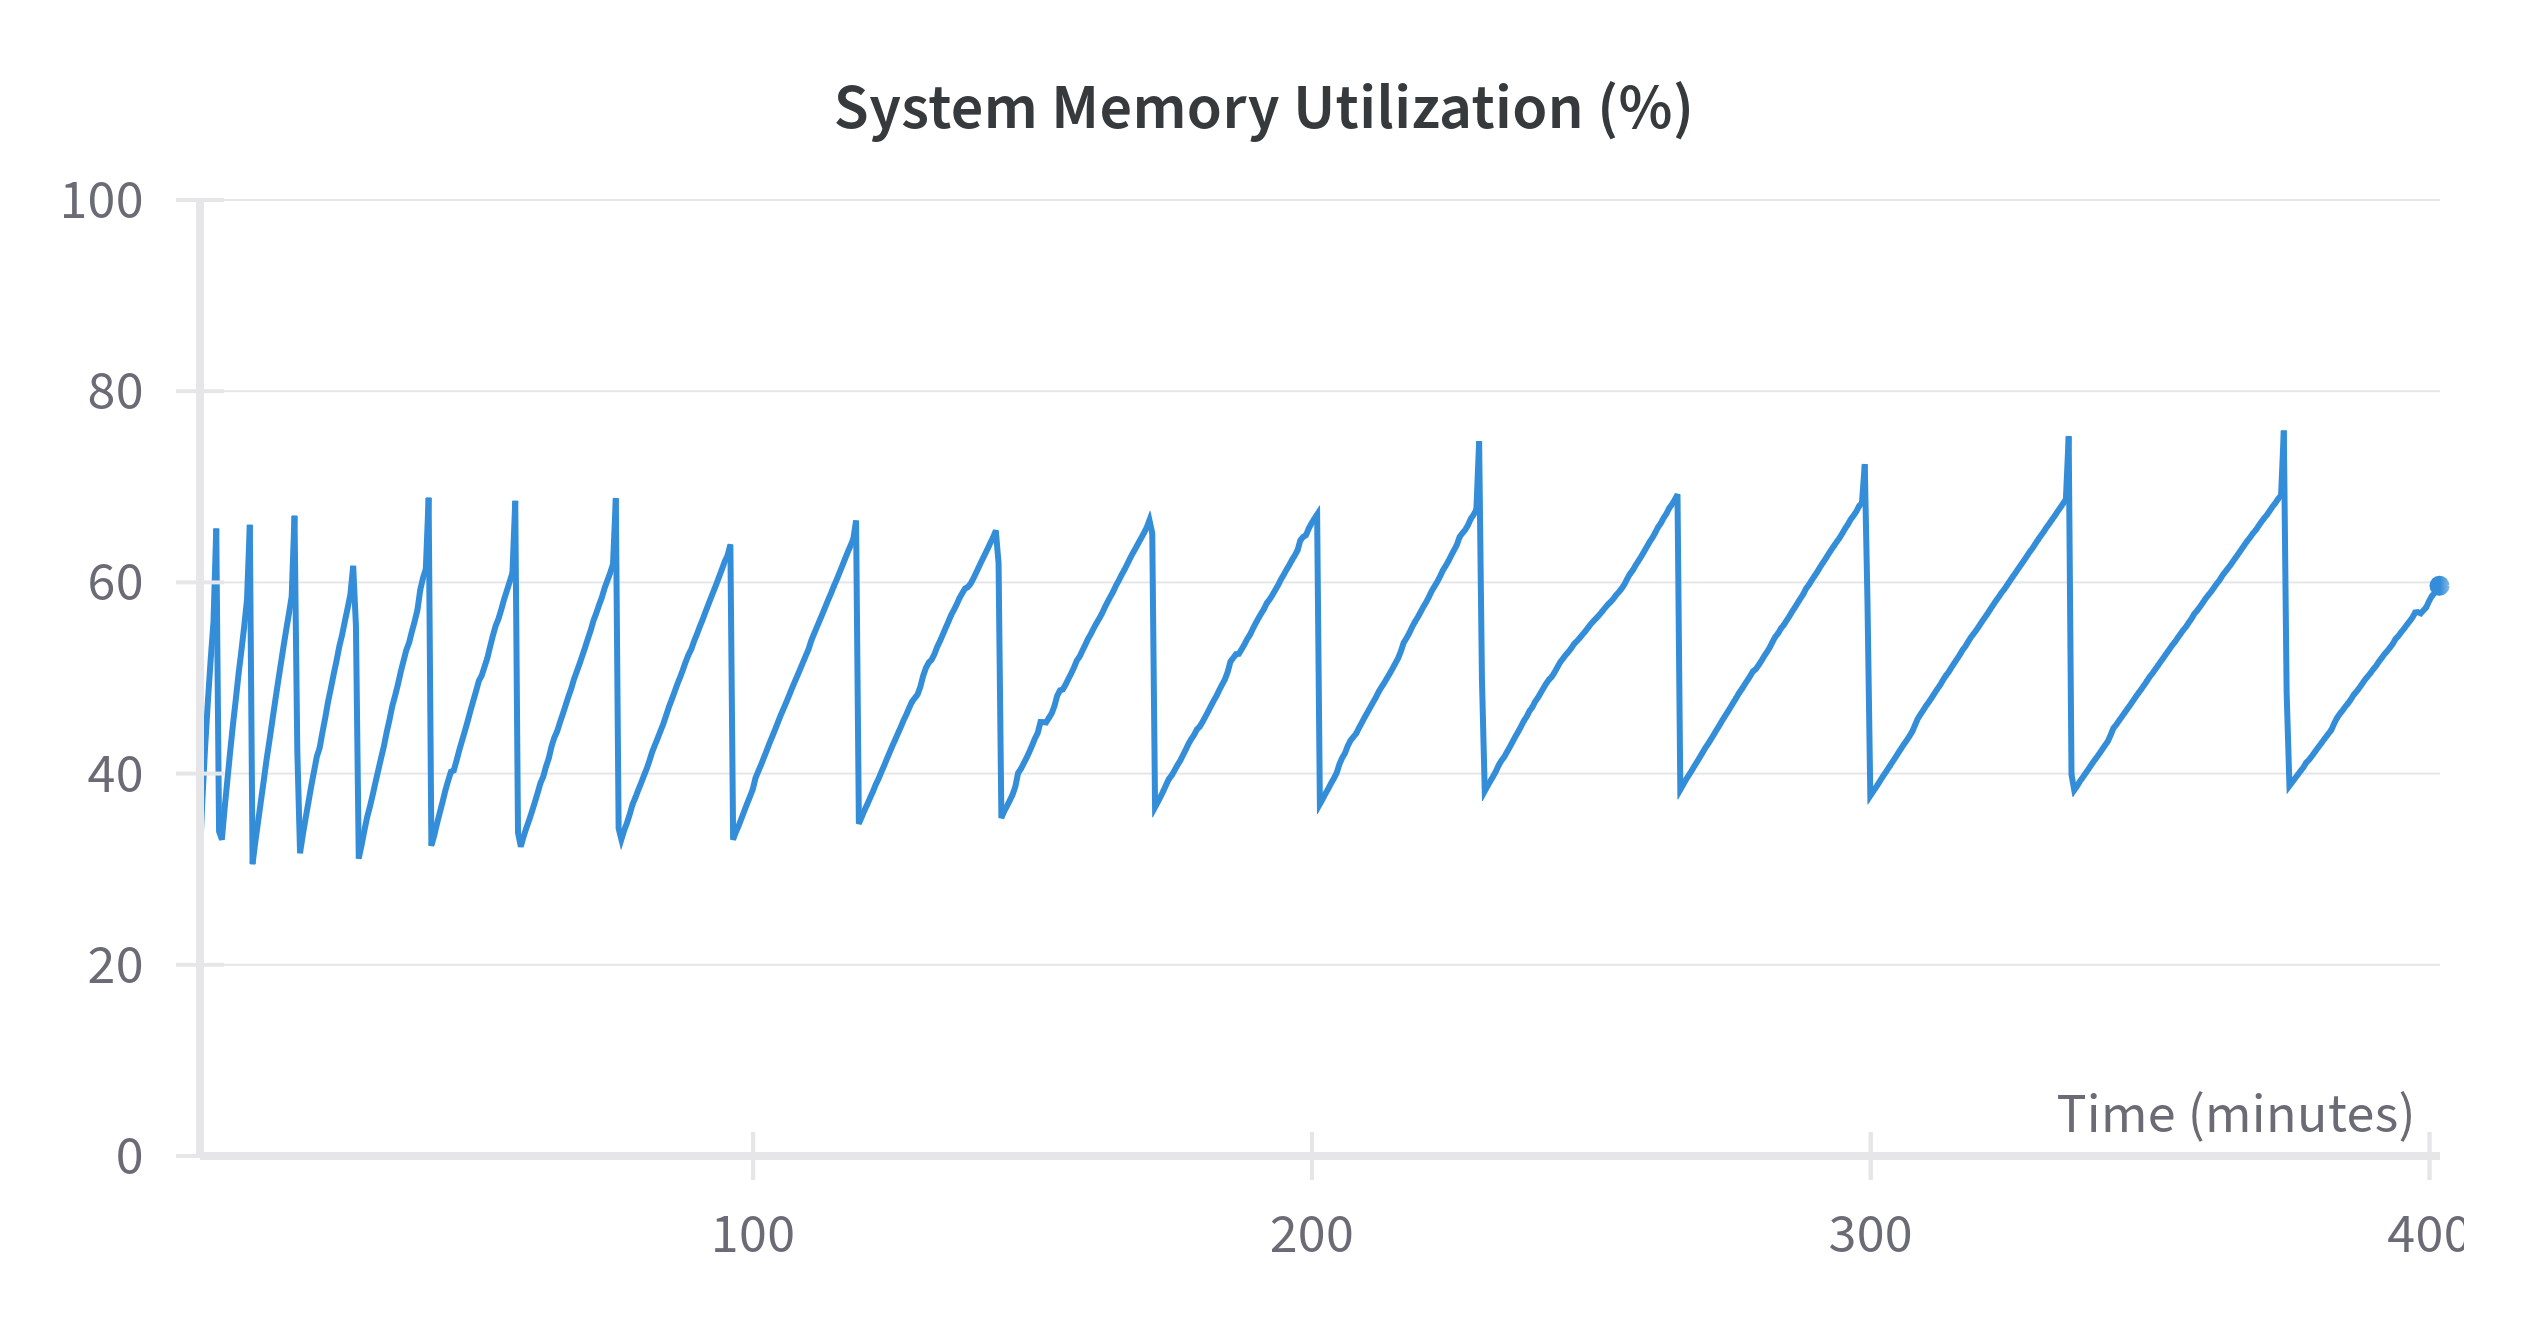
\includegraphics[width=0.8\textwidth]{figures/System_RAM_Utilization.png}
    \caption{Total RAM usage while training an agent}
    \label{fig:sys_memory_useage}
\end{figure}

From the three figures above, it can be seen that the GPU Utilization was low, with a maximum of 42.47\% peak usage. The CPU usage was also low, with a maximum of 4.71\% peak usage, while the Total RAM usage while training the agent was quite high, with a maximum of 75.82\% peak usage. The values provided in the figures above were taken from the wandb system monitor that was running while trianing the agents. In addition, these values have the possibility of being marginally skewed as the hardware running the training the agents was also running visual studio code and other system operating system essential processes. However, it is very evident that RAM was the bottleneck in training the agents. It was possible to train with an additional instance of the environment making the total instances 12, however there was a high chance that the system would crash. This occured while training the agent using the PPO algorithm after 4-5 hour. 

\subsection{data recording}

